\documentclass[12pt, letterpaper]{article}
\usepackage{xcolor}
\usepackage{amsmath}
\usepackage{tikz}
\title{The Length of an Arc}
\begin{document}
\maketitle



\hrulefill

\section{Introduction}
\textcolor{blue}{"Whenever you're trying to calculate something that you can approximate as a sum of a bunch of tiny things}\textcolor{brown}{, 
always try and use an integral." - Grant Sanderson}

Many times when solving problems it is useful to know the length of a curve. 

\section{Derivation}

We already know how to calculate the length of a straight line using the Pythagorean theorem
\begin{equation}
    \text{Length of a straight line} = \sqrt{(x_2 - x_1)^2 + (y_2 - y_1)^2}
\end{equation}



We can first start by splitting our surve into small segments of width $\Delta x$
Since we also know the derivative of the function we can now approximate a small portion of the curve with a straight line

\begin{align}
    \text{Slope of line at x} &= \frac{dy}{dx} = f'(x) \\
    \text{Change in y at x} &= \frac{dy}{dx} \cdot dx = f'(x) dx \\
\end{align}

Since we now know the change in y and the change in x, we can now use the pythagorean theorem to calculate the length of small portion of the line

\begin{align}
    \text{Length of a segment} &= \sqrt{dx^2 + (f'(x) \cdot dx)^2} 
\end{align}

We want to find the sum of all these lengths, but before we can factor out the $\Delta x$ we need to simplify the equation

\begin{align}
    \text{Length of a segment} &= \sqrt{dx^2 + f'(x)^2 \cdot dx^2} \\
    &= \sqrt{1 + f'(x)^2} \cdot dx
\end{align}

Now we can integrate this function over an interval $[a, b]$ and this gives us the formula for the length of a curve

\begin{align}
    \text{Length of a curve} &= \int_{a}^{b} \sqrt{1 + f'(x)^2} \cdot dx
\end{align}

\section{Practice}
1. Find the arc length of a unit semicircle (since we know the formula for the perimeter of a circle we know our answer should be $\frac{2\pi (1)}{2} = \pi$)
\begin{align}
    f(x) &= \sqrt{1-x^2} \\
    \text{Arc length} &= \int_{-1}^{1} \sqrt{1 + f'(x)^2} dx 
\end{align}

\begin{center}
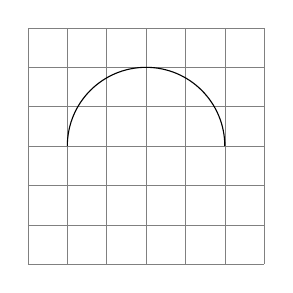
\begin{tikzpicture}
    \draw[step = 0.5cm, gray, very thin] (-1.5,-1.5) grid (1.5,1.5);
    \draw (-1,0) arc (180:0:1cm);
\end{tikzpicture}
\end{center}

\vspace{0.5cm}

2. Find the arc length of $\log(\sec(x))$ from $-\frac{\pi}{4}$ to $\frac{\pi}{4}$

\section{"Difficulties"}
3. Find the arc length of an ellipse
\begin{align}
    f(x) &= \sqrt{1-\frac{x^2}{9}} \\
    f'(x) &= \frac{-\frac{2x}{9}}{2\sqrt{1-\frac{x^2}{9}}}
\end{align}

\begin{center}
    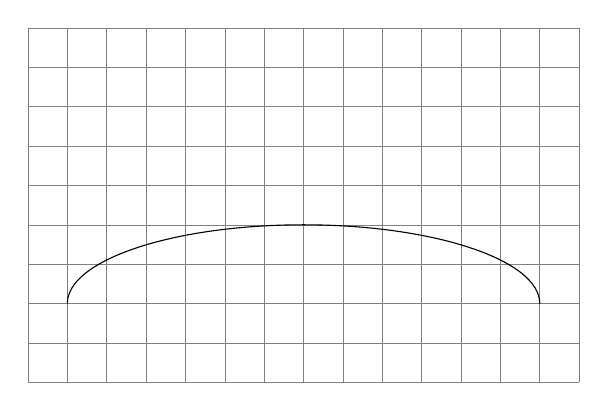
\begin{tikzpicture}
        \draw[step = 0.5cm, gray, very thin] (-3.5,-1) grid (3.5,3.5);
        \draw (-3,0) arc (180:0:3cm and 1cm); 
    \end{tikzpicture}
    \end{center}

\end{document}